\documentclass{article}
\usepackage{fullpage}
\usepackage[utf8]{inputenc}
\usepackage{pict2e}
\usepackage{amsmath}
\usepackage{enumitem}
\usepackage{eurosym}
\usepackage{mathtools}
\usepackage{amssymb, amsfonts, latexsym, cancel}
\setlength{\parskip}{0.3cm}
\usepackage{graphicx}
\usepackage{fontenc}
\usepackage{slashbox}
\usepackage{setspace}
\usepackage{gensymb}
\usepackage{accents}
\usepackage{adjustbox}
\setstretch{1.35}
\usepackage{bold-extra}
\usepackage[document]{ragged2e}
\usepackage{subcaption}
\usepackage{tcolorbox}
\usepackage{xcolor, colortbl}
\usepackage{wrapfig}
\usepackage{empheq}
\usepackage{array}
\usepackage{parskip}
\usepackage{arydshln}
\graphicspath{ {images/} }
\renewcommand*\contentsname{\color{black}Índice} 
\usepackage{array, multirow, multicol}
\definecolor{lightblue}{HTML}{007AFF}
\usepackage{color}
\usepackage{etoolbox}
\usepackage{listings}
\usepackage{mdframed}
\setlength{\parindent}{0pt}
\usepackage{underscore}
\usepackage{hyperref}
\usepackage{tikz}
\usepackage{tikz-cd}
\usetikzlibrary{shapes, positioning, patterns}
\usepackage{tikz-qtree}
\usepackage{biblatex}
\usepackage{pdfpages}
\usepackage{pgfplots}
\usepackage{pgfkeys}
\addbibresource{biblatex-examples.bib}
\usepackage[a4paper, left=1cm, right=1cm, top=1cm,
bottom=1.5cm]{geometry}
\usepackage{titlesec}
\usepackage{titletoc}
\usepackage{tikz-3dplot}
\usepackage{kbordermatrix}
\usetikzlibrary{decorations.pathreplacing}
\newcommand{\Ej}{\textcolor{lightblue}{\underline{Ejemplo}}}
\setlength{\fboxrule}{1.5pt}

% Configura el formato de las secciones utilizando titlesec
\titleformat{\section}
{\color{red}\normalfont\LARGE\bfseries}
{Tema \thesection:}
{10 pt}
{}

% Ajusta el formato de las entradas de la tabla de contenidos
\addtocontents{toc}{\protect\setcounter{tocdepth}{4}}
\addtocontents{toc}{\color{black}}

\titleformat{\subsection}
{\normalfont\Large\bfseries\color{red}}{\thesubsection)}{1em}{\color{lightblue}}

\titleformat{\subsubsection}
{\normalfont\large\bfseries\color{red}}{\thesubsubsection)}{1em}{\color{lightblue}}

\newcommand{\bboxed}[1]{\fcolorbox{lightblue}{lightblue!10}{$#1$}}
\newcommand{\rboxed}[1]{\fcolorbox{red}{red!10}{$#1$}}

\DeclareMathOperator{\N}{\mathbb{N}}
\DeclareMathOperator{\Z}{\mathbb{Z}}
\DeclareMathOperator{\R}{\mathbb{R}}
\DeclareMathOperator{\Q}{\mathbb{Q}}
\DeclareMathOperator{\K}{\mathbb{K}}
\DeclareMathOperator{\im}{\imath}
\DeclareMathOperator{\jm}{\jmath}
\DeclareMathOperator{\col}{\mathrm{Col}}
\DeclareMathOperator{\fil}{\mathrm{Fil}}
\DeclareMathOperator{\rg}{\mathrm{rg}}
\DeclareMathOperator{\nuc}{\mathrm{nuc}}
\DeclareMathOperator{\dimf}{\mathrm{dimFil}}
\DeclareMathOperator{\dimc}{\mathrm{dimCol}}
\DeclareMathOperator{\dimn}{\mathrm{dimnuc}}
\DeclareMathOperator{\dimr}{\mathrm{dimrg}}
\DeclareMathOperator{\dom}{\mathrm{Dom}}
\DeclareMathOperator{\infi}{\int_{-\infty}^{+\infty}}
\newcommand{\dint}[2]{\int_{#1}^{#2}}

\newcommand{\bu}[1]{\textcolor{lightblue}{\underline{#1}}}
\newcommand{\lb}[1]{\textcolor{lightblue}{#1}}
\newcommand{\db}[1]{\textcolor{blue}{#1}}
\newcommand{\rc}[1]{\textcolor{red}{#1}}
\newcommand{\tr}{^\intercal}

\renewcommand{\CancelColor}{\color{lightblue}}

\newcommand{\dx}{\:\mathrm{d}x}
\newcommand{\dt}{\:\mathrm{d}t}
\newcommand{\dy}{\:\mathrm{d}y}
\newcommand{\dz}{\:\mathrm{d}z}
\newcommand{\dth}{\:\mathrm{d}\theta}
\newcommand{\dr}{\:\mathrm{d}\rho}
\newcommand{\du}{\:\mathrm{d}u}
\newcommand{\dv}{\:\mathrm{d}v}
\newcommand{\tozero}[1]{\cancelto{0}{#1}}
\newcommand{\lbb}[2]{\textcolor{lightblue}{\underbracket[1pt]{\textcolor{black}{#1}}_{#2}}}
\newcommand{\dbb}[2]{\textcolor{blue}{\underbracket[1pt]{\textcolor{black}{#1}}_{#2}}}
\newcommand{\rub}[2]{\textcolor{red}{\underbracket[1pt]{\textcolor{black}{#1}}_{#2}}}

\author{Francisco Javier Mercader Martínez}
\date{}
\title{Academia Optativa}
\everymath{\displaystyle}
\newcommand{\vare}{\varepsilon}

\begin{document}
\maketitle
\begin{enumerate}[label=\color{red}\textbf{\arabic*)}, leftmargin=*]
	\item \lb{Calcular y representar el dominio de la siguiente función: \[ f(x,y)=\ln(9-x^2-y^2) \]}
	Como sabemos, lo de dentro de un logaritmo neperiano nunca puede ser negativo ni 0, por eso: \[ 0-x^2-y^2>0\longrightarrow9>x^2+y^2 \]Por lo tanto, podemos representar el dominio como: $\bboxed{\dom(f)=\left\{(x,y)\in\R^2 \arrowvert x^2+y^2<9\right\}}$
	
	\fbox{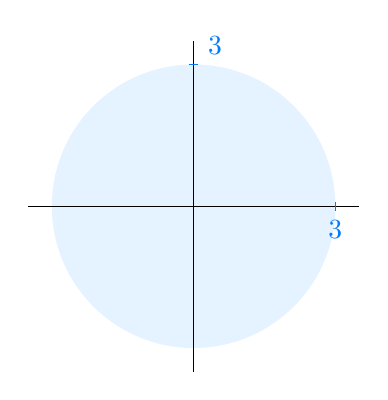
\begin{tikzpicture}[scale=0.6, baseline=(current bounding box.center)]
	\fill[lightblue!10] (0,0) circle (3);
	\draw (-3.5,0) -- (3.5,0);
	\draw (0,-3.5) -- (0,3.5);
	\draw[lightblue] (-0.1,3) -- (0.1,3) node[above right] {$3$};
	\draw[lightblue] (3,0.1) -- (3,-0.1) node[below] {$3$};
	\end{tikzpicture}}\qquad\begin{minipage}[l]{0.4\textwidth}
	Este recinto representa el interior de la circunferencia de centro $(0,0)$ y radio $R=3$.
	\end{minipage}
	\item \lb{Calcular y representar el dominio de la siguiente función: \[ f(x,y)=\sqrt{4-x^2}\cdot\sqrt{9-y^2} \]}
	
	\begin{minipage}{0.45\textwidth}
	Como dentro de una raíz solo puede haber elementos que sean positivos o cero: 
	
	\begin{itemize}
	\item $4-x^2\ge0\longrightarrow x^2\le4\longrightarrow-2\le x\le 2$
	\item $9-y^2\ge0\longrightarrow y^2\le9\longrightarrow-3\le y\le3$
	\end{itemize}
	
	$\bboxed{\dom(f)=\left\{(x,y)\in\R^2 \arrowvert -2\le x\le2,\:-3\le y\le3\right\}}$
	\end{minipage}\qquad\begin{minipage}{0.45\textwidth}
		\fbox{
		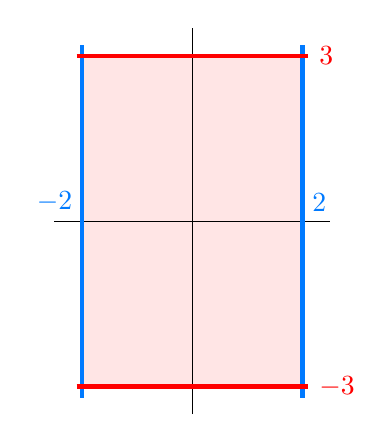
\begin{tikzpicture}[scale=0.7]
		\fill[red!10] (-2,3) rectangle (2,-3);
		\draw (-2.5,0) -- (2.5,0);
		\draw (0,-3.5) -- (0,3.5);
		\foreach \x in {-2,2}{
		\draw[lightblue, line width=1.5] (\x,-3.2) -- (\x,3.2);
		}
		\foreach \y in {-3,3}{
		\draw[red, line width=1.5] (-2.1,\y) -- (2.1,\y) node[right] {$\y$};
		}
		\node[lightblue, above left] at (-2,0) {$-2$};
		\node[lightblue, above right] at (2,0) {$2$};
		\end{tikzpicture}
		}
		\end{minipage}
		
		\item \lb{Realizar el límite direccional mediante el cambio de rectas de: \[ \lim_{(x,y)\to(0,0)}\dfrac{xy^2}{x^2+y^2} \]}
		
		$\lim_{(x,y)\to(0,0)}\dfrac{xy^2}{x^2+y^2}=\left\{\begin{array}{l}
		y-b=m(x-a)\\
		y=mx
		\end{array}\right\}=\lim_{x\to0}\dfrac{x\cdot m^2x^2}{x^2+m^2x^2}=\lim_{x\to0}\dfrac{m^2\cdot x^{\cancel{3}}}{\cancel{x^2}(1+m^2)}=\lim_{x\to0}\dfrac{m^2x}{1+m^2}=0$
		
		No sabemos si existe el límite pero en caso de existir valdría $L=0$.
		
		\item \lb{Realizar el límite direccional mediante el cambio de rectas de: \[ \lim_{(x,y)\to(0,0)}\dfrac{xy}{x^2+y^2} \]}
		
		$\lim_{(x,y)\to(0,0)}\dfrac{xy}{x^2+y^2}=\left\{y=mx\right\}=\lim_{x\to0}\dfrac{xmx}{x^2+m^2x^2}=\lim_{x\to0}\dfrac{m\cdot\cancel{x^2}}{\cancel{x^2}(m^2+1)}=\dfrac{m}{1+m^2}$
		
		Como el resultado depende de $m$, entonces \underline{no existe el límite}.
		
		\item \lb{Realizar el límite direccional mediante rectas y parábolas en el siguiente límite: \[ \lim_{(x,y)\to(0,0)}\dfrac{x^3+y^3}{x^2+y^2} \]}
		\underline{Rectas:}
		
		$\lim_{(x,y)\to(0,0)}\dfrac{x^3+y^3}{x^2+y^2}=\left\{y=mx\right\}=\lim_{x\to0}\dfrac{x^3+m^3x^3}{x^2+m^2x^2}=\lim_{x\to0}\dfrac{x^{\cancel{3}}(1+m^3)}{\cancel{x^2}(1+m^2)}=\lim_{x\to0}\dfrac{x(1+m^3)}{1+m^2}=0$
		
		No sabemos si existe el límite, pero en caso de existir valdría $L=0$.
		
		\underline{Parábolas:}
		
		$\lim_{(x,y)\to(0,0)}\dfrac{x^3+y^3}{x^2+^2}=\left\{y=mx^2\right\}=\lim_{x\to0}\dfrac{x^3+m^3x^6}{x^2+m^3x^4}=\lim_{x\to0}\dfrac{x^{\cancel{3}}(1+m^3x^3)}{\cancel{x^2}(1+m^2x^2)}=\lim_{x\to0}\dfrac{1+m^3x^3}{1+m^2x^2}=0$
		
		No sabemos si existe el límite, pero en caso de existir valdría $L=0$.
		\item \lb{Dado el siguiente límite \[ \lim_{(x,y)\to(0,0)}\dfrac{xy^2}{x^2+y^4} \]}
		\begin{enumerate}[label=\color{red}\alph*)]
			\item \db{Calcular su límite direccional por rectas.}
			
			$\lim_{(x,y)\to(0,0)}\dfrac{xy^2}{x^2+y^4}=\left\{y=mx\right\}=\lim_{x\to0}\dfrac{xm^2x^2}{x^2+m^4x^4}=\lim_{x\to0}\dfrac{m^2x^{\cancel{3}}}{\cancel{x^2}(1`m^4x^2)}$
			\item \db{Calcular su límite direccional por parábolas}
			
			$\lim_{(x,y)\to(0,0)}\dfrac{xy^2}{x^2+y^4}=\left\{y=mx^2\right\}=\lim_{x\to0}\dfrac{xm^2x^4}{x^2+m^4x^8}=\lim_{x\to0}\dfrac{m^2x^{\cancel{5}}}{\cancel{x^2}(1+m^4x^6)}=\lim_{x\to0}\dfrac{m^2x^3}{1+m^4x^6}=\dfrac{0}{1}=0$
			
			No sabemos si existe el límite, pero en caso de existir valdría $0$.
			\item \db{Calcular su límite direccional por aquel cambio que consideres óptimo.}
			
			Como sabemos, el cambio óptimo en límites direccionales, es aquel que nos deja igualados los grados de los términos del denominador: \[ \lim_{(x,y)\to(0,0)}\dfrac{xy^2}{x^2+y^4}=\left\{x=my^2\right\}=\lim_{y\to0}\dfrac{my^2\cdot y^2}{m^2y^4+y^4}=\lim_{y\to0}\dfrac{m\cdot\cancel{y^4}}{\cancel{y^4}(m^2+1)}=\dfrac{m}{m^2+1} \]
			Como depende de $m$, podemos asegurar que \underline{no} existe el límite.
		\end{enumerate}
		\item \lb{Comprobar si existe el siguiente límite: \[ \lim_{(x,y)\to(0,0)}\dfrac{xy^3}{x^2+y^6} \]}
		Comenzamos realizando los límites direccionales: \[ \lim_{(x,y)\to(0,0)}\dfrac{xy^3}{x^2+y^6}=\left\{x=my^3\right\}=\lim_{y\to0}\dfrac{my^3\cdot y^3}{m^2y^6+y^6}=\lim_{y\to0}\dfrac{m\cancel{y^6}}{\cancel{y^6}(m^2+1)}=\dfrac{m}{m^2+1} \]
		Como depende de $m$ que es la dirección de acercamiento, entonces \underline{no} existe el límite.
		\item \lb{Comprobar la existencia del siguiente límite mediante el cambio de coordenadas polares. \[ \lim_{(x,y)\to(0,0)}\dfrac{xy}{x^2+y^2} \]}
		$\lim_{(x,y)\to(0,0)}\dfrac{xy}{x^2+y^2}=\left\{\begin{array}{l}
		x=\rho\cos\theta\\
		y=\rho\sin\theta
		\end{array}\right\}=\lim_{\rho\to0}\dfrac{\rho\cos\theta\cdot\rho\sin\theta}{\rho^2\cos^2\theta+\rho^2\sin^2\theta}=\dfrac{\cancel{\rho^2}\cos\theta\sin\theta}{\cancel{\rho^2}\underset{\begin{subarray}{c}
		\rotatebox{90}{=}\\
		1
		\end{subarray}}{(\cos\theta+\sin\theta)}}=\cos\theta\cdot\sin\theta$
		
		Como el resultado depende de $\theta$ que es la dirección de acercamiento, entonces \underline{no} existe el límite.
		
		\item \lb{Calcular el siguiente límite mediante límites iterados: \[ \lim_{(x,y)\to(0,0)}\dfrac{x^3+y^3}{x^2+y^2} \]}
		\begin{itemize}
		\item $\lim_{y\to0}\left(\lim_{x\to0}\dfrac{\cancel{x^3}+y^3}{\cancel{x^2}+y^2}\right)=\lim_{y\to0}\dfrac{y^{\cancel{3}}}{\cancel{y^2}}=\lim_{y\to0}y=0$
		\item $\lim_{x\to0}\left(\lim_{y\to0}\dfrac{x^3+\cancel{y^3}}{x^2+\cancel{y^2}}\right)=\lim_{x\to0}\dfrac{x^{\cancel{3}}}{\cancel{x^2}}=\lim_{x\to0}x=0$
		\end{itemize}
		No sabemos si existe el límite, pero en caso de existir valdría 0.
		\item \lb{Calcular los límites iterados del siguiente límite: \[ \lim_{(x,y)\to(0,0)}\dfrac{x^3+3y^2}{x^2+y^2} \]}
		\begin{itemize}
		\item $\lim_{y\to0}\left(\lim_{x\to0}\dfrac{\cancel{x^3}+3y^2}{\cancel{x^2}+y^2}\right)=\lim_{y\to0}\dfrac{3y^2}{y^2}=3$
		\item $\lim_{x\to0}\left(\lim_{y\to0}\dfrac{x^3+\cancel{3y^2}}{x^2+\cancel{y^2}}\right)=\lim_{x\to0}\dfrac{x^{\cancel{3}}}{\cancel{x^2}}=\lim_{x\to0}x=0$
		\end{itemize}
		Como los límites no coinciden entonces \underline{no} existe el límite.
		
		\item \lb{Estudiar la existencia del límite en el punto $(0,0)$ de la función $f:\R^2\backslash\{(0,0)\}\longrightarrow\R$ dada por \[ f(x,y)=\dfrac{x^2+y}{\sqrt{x^2+y^2}}. \]}
		\begin{enumerate}[label=\arabic*)]
			\item \underline{Límites direccionales:} \[ \lim_{(x,y)\to(0,0)}\dfrac{x^2+y}{\sqrt{x^2+y^2}}=\left\{y=mx\right\}=\lim_{x\to0}\dfrac{x^2+mx}{\sqrt{x^2+m^2x^2}}=\lim_{x\to0}\dfrac{x(x+m)}{\sqrt{x^2(1+m^2)}}=\lim_{x\to0}\dfrac{\cancel{x}(x+m)}{\cancel{x}\sqrt{1+m^2}}=\lim_{x\to0}\dfrac{x+m}{\sqrt{1+m^2}}=\dfrac{m}{\sqrt{1+m^2}}\]
			Como depende de $m$ entonces no existe el límite.
			
			Por lo tanto: $\nexists\lim_{(x,y)\to(0,0)}\dfrac{x^2+y}{\sqrt{x^2+y^2}}$
		\end{enumerate}
		\item \lb{Estudiar la existencia del límite en el punto $(0,0)$ de la función $\vec{f}:\R^2\backslash\{(0,0)\}\longrightarrow\R^2$ definida por \[ \vec{f}(x,y)=\left(x+y^2,\dfrac{xy}{x^2+y^2}\right). \]}
		Como podemos observar la función $\vec{f}(x,y)$ es una función vectorial, ya que su imagen es un vector, en este caso, de dos coordenadas.
		
		Para que una función vectorial tenga límite, debe verificarse que todas sus funciones coordenadas tengan límite.
		
		Vamos a empezar por \[ \lim_{(x,y)\to(0,0)}\dfrac{xy}{x^2+y^2}=\{y=mx\}=\lim_{x\to0}\dfrac{xmx}{x^2+m^2x^2}=\lim_{x\to0}\dfrac{m\cancel{x^2}}{\cancel{x^2}(1+m^2)}=\dfrac{m}{1+m^2}\longrightarrow\nexists\lim \]
		Por lo tanto, como una de las coordenadas no tiene límite, entonces decimos que la función no tiene límite.
		\item \lb{Estudiar la existencia del límite en el punto $(0,0)$ de la función $f:\R^2\backslash\{(0,0)\}\longrightarrow\R$ dada por \[ f(x,y)=\dfrac{x^4+3x^2y^2+2xy^3}{(x^2+y^2)^2}. \]}
		\begin{enumerate}[label=\arabic*)]
			\item \underline{Límites direccionales:}
			
			$\lim_{(x,y)\to(0,0)}\dfrac{x^4+3x^2y^2+2xy^3}{x^2+y^2}=\{y=mx\}=\lim_{x\to0}\dfrac{x^4+3x^2m^2x^2+2xm^3x^3}{(x^2+m^2x^2)^2}=\lim_{x\to0}\dfrac{x^4+3m^2x^4+2m^3x^4}{(x^2(1+m^2))^2}=\lim_{x\to0}\dfrac{\cancel{x^4}(1+3m^2+2m^3)}{\cancel{x^4}(1+m^2)^2}=\dfrac{1+3m^2+2m^3}{(1+m^2)^2}$
			
			No existe el límite porque depende de $m$.
			
		\end{enumerate}
		\item \lb{Estudiar la existencia del límite en el punto $(0,0)$ de la función $f:\R^2\backslash\{(0,0)\}\longrightarrow\R$ dada por \[ f(x,y)=\dfrac{xy^2}{x^2+y^4}. \]}
			\begin{enumerate}[label=\arabic*)]
				\item \underline{Límites direccionales:} \[ \lim_{(x,y)\to(0,0)}\dfrac{xy^2}{x^2+y^4}=\{x=my^2\}=\lim_{y\to0}\dfrac{my^2\cdot y^2}{m^2y^4+y^4}=\lim_{y\to0}\dfrac{m\cancel{y^4}}{\cancel{y^4}(m^2+1)}=\dfrac{m}{m^2+1} \] No existe el límite porque depende de $m$.
			\end{enumerate}
		\item \lb{¿Qué tiene que valer el número real $k$ para que la función \[ f(x,y)=\begin{cases}
		\dfrac{y^2}{x^2+y^2} & \text{si }(x,y)\neq(0,0),\\
		k & \text{si }(x,y)=(0,0).
		\end{cases} \] sea continua?}
		
		El número real $k$, que es $f(0,0)=k$, para que sea continua, deberá valer lo mismo que valga el límite de la función en el punto $(0,0)$, para que casi coincidan y por lo tanto sea continua.
		
		Hagamos por lo tanto el límite de $f(x,y)$ en el punto $P(0,0)$:
		\begin{enumerate}[label=\arabic*)]
			\item \underline{Límites direccionales:} \[ \lim_{(x,y)\to(0,0)}\dfrac{y^2}{x^2+y^2}=\{y=mx\}=\lim_{x\to0}\dfrac{m^2x^2}{x^2+m^2x^2}=\lim_{x\to0}\dfrac{m^2\cancel{x^2}}{\cancel{x^2}(1+m^2)}=\dfrac{m^2}{1+m^2} \]No existe el límite, pues el resultado depende de $m$.
		\end{enumerate}
		Por lo tanto, al no haber límite en $(0,0)$, no existe ningún valor de $k$, que haga que la función sea continua en $(0,0)$.
		\item \lb{Estudiar la existencia del siguiente límite: \[ \lim_{(x,y)\to(0,0)}\dfrac{xy^4}{x^2+y^8} \]}
		
		$\lim_{(x,y)\to(0,0)}\dfrac{xy^4}{x^2+y^8}=\{x=my^4\}=\lim_{y\to0}\dfrac{my^4\cdot y^4}{m^2y^8+y^8}=\lim_{y\to0}\dfrac{m\cancel{y^8}}{\cancel{y^8}(m^2+1)}=\dfrac{m}{m^2+1}\quad\nexists\lim$ porque depende de $m$.
		\item \lb{Estudiar la existencia del siguiente límite, y calcularlo en caso de que exista: \[ \lim_{(x,y)\to(0,0)}\dfrac{x^3}{x^2+y^2} \]}
		\begin{enumerate}[label=\arabic*), leftmargin=*]
			\item \underline{Límites direccionales:} \[ \lim_{(x,y)\to(0,0)}\dfrac{x^3}{x^2+y^2}=\{y=mx\}=\lim_{x\to0}\dfrac{x^3}{x^2+m^2x^2}=\lim_{x\to0}\dfrac{x^{\cancel{3}}}{\cancel{x^2}(1+m^2)}=\lim_{x\to0}\dfrac{x}{1+m^2}=0 \] No sabemos si existe el límite, pero en caso de existir valdrá 0.
			\item \underline{Límites por cambio de coordenadas polares:}
			
			$\lim_{(x,y)\to(0,0)}\dfrac{x^3}{x^2+y^2}=\left\{\begin{array}{l}
			x=\rho\cos\theta\\
			y=\rho\sin\theta
			\end{array}\right\}=\lim_{\rho\to0}\dfrac{\rho^3\cos^3\theta}{\rho^2\cos^2\theta+\rho^2\sin^2\theta}=\lim_{\rho\to0}\dfrac{\rho^{\cancel{3}}\cos^3\theta}{\cancel{\rho^2}\underset{\begin{subarray}{c}
			\rotatebox{90}{=}\\
			1
			\end{subarray}}{(\cos^2\theta+\sin^2\theta)}}=\linebreak\lim_{\rho\to0}\rho\cos^3\theta=0$
			\item \underline{Límite iterados o reiterados:}
			\begin{itemize}
			\item $\lim_{y\to0}\left(\lim_{x\to0}\dfrac{x^3}{x^2+y^2}\right)=\lim_{y\to0}0=0$
			\item $\lim_{x\to0}\left(\lim_{y\to0}\dfrac{x^3}{x^2+\tozero{y^2}}\right)=\lim_{x\to0}\dfrac{x^{\cancel{3}}}{\cancel{x^2}}=\lim_{x\to0}x=0$
			\end{itemize}
			Hemos suspendido las tres pruebas, quedándonos como candidato al límite el valor $L=0$.
			\item \underline{Definición de límite:} 
			
			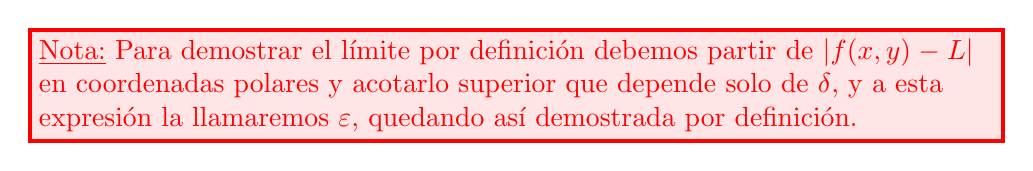
\begin{tikzpicture}
				\node[red, draw=red, fill=red!10, line width=1.5, text width=\linewidth] {\underline{Nota:} Para demostrar el límite por definición debemos partir de $|f(x,y)-L|$ en coordenadas polares y acotarlo superior que depende solo de $\delta$, y a esta expresión la llamaremos $\varepsilon$, quedando así demostrada por definición.};
			\end{tikzpicture}
			
			\[ \forall\varepsilon>0\quad\exists\delta>0/\left|f(x,y)-L\right|<\varepsilon\text{ si }\left\|(x,y)-(0,0)\right\|<\delta\] en coordenadas polares: \[ \forall\varepsilon>0\quad\exists\delta>0/|\rho\cos^3\theta-0|<\varepsilon\text{ si }\rho<\delta \] $|\rho\cos^3\theta-0|=|\rho\cos^3\theta|=\rho\cdot|\cos\theta|^3\le\rho<\boxed{\delta=\varepsilon}$
			
			Por lo tanto, existe el límite y vale 0: $\bboxed{\lim_{(x,y)\to(0,0)}\dfrac{x^3}{x^2+y^2}=0}$
		\end{enumerate}
		\item \lb{Estudiar la existencia del límite en el punto $(0,0)$ de la función $f:\R^2\backslash\{(0,0)\}\longrightarrow\R$ dada por \[ f(x,y)=\dfrac{x^4+y^4}{x^2+y^2}. \]}
		\begin{enumerate}[label=\arabic*)]
			\item \underline{Límites direccionales:} \[ \lim_{(x,y)\to(0,0)}\dfrac{x^4+y^4}{x^2+y^2}=\{y=mx\}=\lim_{x\to0}\dfrac{x^4+m^4x^4}{x^2+m^2x^2}=\lim_{x\to0}\dfrac{x^{\cancel{4}}(1+m^4)}{\cancel{x^2}(1+m^2)}=\lim_{x\to0}\dfrac{x^2(1+m^4)}{1+m^2}=0 \]No sabemos si existe el límite pero en caso de existir valdrá 0.
			\item \underline{Límites por cambio de coordendas polares:} 
			
			$\lim_{(x,y)\to(0,0)}\dfrac{x^4+y^4}{x^2+y^2}=\left\{\begin{array}{l}
			x=\rho\cos\theta\\
			y=\rho\sin\theta
			\end{array}\right\}=\lim_{\rho\to0}\dfrac{\rho^4\cos^4\theta+\rho^4\sin^4\theta}{\rho^2\cos^2\theta+\rho^2\sin^2\theta}=\lim_{\rho\to0}\dfrac{\rho^{\cancel{4}}(\cos^4\theta+\sin^4\theta)}{\cancel{\rho^2}\underset{\begin{subarray}{c}
			\rotatebox{90}{=}\\
			1
			\end{subarray}}{(\cos^2\theta+\sin^2\theta)}}=\linebreak\lim_{\rho\to0}\rho^2(\cos^4\theta+\sin^4\theta)=0$
			\item \underline{Límites iterados o reiterados:}
			\begin{itemize}
			\item $\lim_{y\to0}\left(\lim_{x\to0}\dfrac{\cancel{x^4}+y^4}{\cancel{x^2}+y^2}\right)=\lim_{y\to0}\dfrac{y^{\cancel{4}}}{\cancel{y^2}}=\lim_{y\to0}y^2=0$
			\item $\lim_{x\to0}\left(\lim_{y\to0}\dfrac{x^4+\cancel{y^4}}{x^2+\cancel{y^2}}\right)=\lim_{x\to0}\dfrac{x^{\cancel{4}}}{\cancel{x^2}}=\lim_{x\to0}x^2=0$
			\end{itemize}
			\item \underline{Definición de límite:} 
			\[ \forall\varepsilon>0\quad\exists\delta>0/|f(x,y)-0|<\varepsilon\text{ si }\overset{\begin{subarray}{c}
			\sqrt{x^2+y^2}\\
			\rotatebox{90}{=}
			\end{subarray}}{\|(x,y)-(0,0)\|}<\delta \]En coordenadas polares será:
			\[ \forall\varepsilon>0\quad\exists\delta>0/|\rho^2(\cos^4\theta+\sin^4\theta)-0|<\varepsilon\text{ si }\rho<\delta \] $|\rho^2(\cos^4\theta+\sin^4\theta)|=\rho^2|\cos^4\theta+\sin^4\theta|\le2\rho^2<\boxed{2\delta^2=\varepsilon}$
			
			Queda demostrada la definición.
		\end{enumerate}
		Por lo tanto, existe el límite: $\bboxed{\lim_{(x,y)\to(0,0)}\dfrac{x^4+y^4}{x^2+y^2}=0}$
		\item \lb{Calcular las derivadas parciales de la siguiente función \[ f(x,y)=x^3+3y^2+xy \]}
		$\bboxed{\begin{cases}
		\frac{\partial f}{\partial x}=3x^2+y\\
		\frac{\partial f}{\partial y}=6y+x
		\end{cases}}$
		\item \lb{Calcular las derivadas parciales de la siguiente función: \[ f(x,y)=\dfrac{x}{x^2+y^2} \]}
		$\begin{array}{l}
		\frac{\partial f}{\partial x}=\dfrac{1+(x^2+y^2)-2x\cdot x}{(x^2+y^2)^2}=\dfrac{-x^2+y^2}{(x^2+y^2)^2}\\
		\frac{\partial f}{\partial y}=\dfrac{0\cdot(x^2+y^2)-2y\cdot x}{(x^2+y^2)^2}=\dfrac{-2xy}{(x^2+y^2)^2}
		\end{array}\longrightarrow\bboxed{\begin{cases}
		\frac{\partial f}{\partial x}=\frac{-x^2+y^2}{(x^2+y^2)^2}\\
		\frac{\partial f}{\partial y}=\frac{-2xy}{(x^2+y^2)^2}
		\end{cases}}$
		\item \lb{Calcular las derivadas parciales de la siguiente función: \[ f(x,y)=e^{x^2+y^3} \]}
		
		$\begin{array}{l}
		\dfrac{\partial f}{\partial x}=e^{x^2+y^3}\cdot2x\\
		\dfrac{\partial f}{\partial y}=e^{x^2+y^3}\cdot3y^2
		\end{array}\longrightarrow\bboxed{\begin{cases}
		\dfrac{\partial f}{\partial x}=e^{x^2+y^3}\cdot2x\\
		\dfrac{\partial f}{\partial y}=e^{x^2+y^3}\cdot3y^2
		\end{cases}}$
		\item \lb{Estudiar la existencia del límite en el punto $(0,0)$ de la función $f:\R^2\backslash\{(0,0)\}\longrightarrow\R$ dada por \[ f(x,y)=\dfrac{2x^5+2y^3(2x^2-y^2)}{(x^2+y^2)^2} \]}
		\begin{enumerate}[label=\arabic*)]
			\item \underline{Límites direccionales:}
			
			$\lim_{(x,y)\to(0,0)}\dfrac{2x^5+2y^3\cdot(2x^2-y^2)}{(x^2+y^2)^2}=\{y=mx\}=\lim_{x\to0}\dfrac{2x^5+4x^5m^5-2m^5x^5}{(x^2+m^2x^2)^2}=\lim_{x\to0}\dfrac{2x^5+4m^5x^5-2m^5x^5}{(x^2(1+m^2))^2}=\lim_{x\to0}\dfrac{x^{\cancel{5}}(2+4m^5-2m^5)}{\cancel{x^4}(1+m^2)^2}=\lim_{x\to0}\dfrac{x(2+4m^5-2m^5)}{(1+m^2)^2}=0$
			
			No sabemos si existe el límite pero en caso de existir valdrá 0.
			\item \underline{Límites por cambio de coordendas polares}
			
			$\lim_{(x,y)\to(0,0)}\dfrac{2x^5+2y^3\cdot(2x^2-y^2)}{(x^2+y^2)^2}=\left\{\begin{array}{l}
			x=\rho\cos\theta\\
			y=\rho\sin\theta
			\end{array}\right\}=\lim_{\rho\to0}\dfrac{2\rho^5\cos^5\theta+4\rho^4\cos^2\theta\rho^3\sin^3\theta-2\rho^5\sin^5\theta}{(\rho^2\cos^2\theta+\rho^2\sin^2\theta)^2}=\linebreak\lim_{\rho\to0}\dfrac{2\rho^5\cos^5\theta+4\rho^5\cos^2\theta\sin^3\theta-2\rho^5\sin^5\theta}{(\rho^2\underset{\begin{subarray}{c}
			\rotatebox{90}{=}\\
			1
			\end{subarray}}{(\cos^2\theta+\sin^2\theta)})^2}=\lim_{\rho\to0}\dfrac{e^{\cancel{5}}(2\cos^5\theta+4\cos^2\theta\sin^3\theta-2\sin^5\theta)}{\cancel{\rho^4}}=\linebreak\lim_{\rho\to0}\rho(2\cos^5\theta+4\cos^2\theta\sin^3\theta-2\sin^5\theta)=0$
			
			No sabemos si existe el límite pero en caso de existir valdrá 0.
			\item \underline{Límites iterados o reiterados}
			\begin{itemize}
			\item $\lim_{y\to0}\left(\lim_{x\to0}\dfrac{\cancel{2x^5}+\cancel{4x^2y^3}-2y^5}{(\cancel{x^2}+y^2)^2}\right)=\lim_{y\to0}\dfrac{-2y^5}{y^4}=\lim_{y\to0}(-2y)=0$
			\item $\lim_{x\to0}\left(\lim_{y\to0}\dfrac{2x^5+\cancel{4x^2y^4}-\cancel{2y^5}}{(x^2\cancel{y^2})^2}\right)=\lim_{x\to0}\dfrac{2x^5}{x^4}=\lim_{x\to0}2x=0$
			\end{itemize}
			Como podemos observar, hemos superado las tres pruebas, por lo tanto nos falta demostrar la definición de límite.
			\item Definición de límite \[ \forall\varepsilon>0\quad\exists\delta>0/|f(x,y)-L|<\varepsilon\text{ si }\|(x,y)-(0,0)\|<\delta \] En coordenadas polares: \[ \forall\varepsilon>0\quad\exists\delta>0/|f(\rho,\theta)-0|<\varepsilon\text{ si }\rho<\delta \]$|f(\rho,\theta)|=|\rho(2\cos^5\theta+4\cos^2\theta-2\sin^5\theta)|=\rho|(2\cos^5\theta+4\cos^2\theta\sin^3\theta-2\sin^5\theta)|\le8\rho<\boxed{8\delta=\varepsilon}$
			
			Queda así demostrada la definición.
			\end{enumerate}
			Por lo tanto, si existe el límite y vale cero $\bboxed{\lim_{(x,y)\to(0,0)}\dfrac{2x^5+2y^3\cdot(2x^2-y^2)}{(x^2+y^2)^2}=0}$
			
		\item \lb{¿Qué tiene que valore el número real $k$ para que la función \[ f(x,y)=\begin{cases}
		\dfrac{x^2y}{x^2+y^2} & \text{si }(x,y)\neq(0,0),\\
		k & \text{si }(x,y)=(0,0).
		\end{cases} \]sea continua?}
		Lo primero que debe ocurrir para que sea continua en $(0,0)$ es que exista el límite. En caso de que así sea, para que sea continua deberemos forzar para que $f(0,0)=k$ coincida con dicho límite. Será así como obtendremos el valor de $k$.
		
		Estudiamos la existencia del límite de $f(x,y)$ en el punto $(0,0)$:
		\begin{enumerate}[label=\arabic*)]
			\item \underline{Límites direccionales:} \[ \lim_{(x,y)\to(0,0)}\dfrac{x^2y}{x^2+y^2}=\{y=mx\}=\lim_{x\to0}\dfrac{x^2\cdot mx}{x^2+m^2x^2}=\lim_{x\to0}\dfrac{mx^{\cancel{3}}}{\cancel{x^2}(1+m^2)}=\lim_{x\to0}\dfrac{mx}{1+m^2}=0 \]No sabemos si existe el límite pero en caso de existir valdrá 0.
			\item \underline{Límite por cambio de corrdenadas polares:}
			
			$\lim_{(x,y)\to(0,0)}\dfrac{x^2y}{x^2+y^2}=\left\{\begin{array}{l}
			x=\rho\cos\theta\\
			y=\rho\sin\theta
			\end{array}\right\}=\lim_{\rho\to0}\dfrac{\rho^2\cos^2\theta\cdot\rho\sin\theta}{\rho^2\cos^2\theta+\rho^2\sin^2\theta}=\lim_{\rho\to0}\dfrac{\rho^{\cancel{3}}(\cos^2\theta\sin\theta)}{\cancel{\rho^2}\underset{\begin{subarray}{c}
			\rotatebox{90}{=}\\
			1
			\end{subarray}}{(\cos^2\theta+\sin^2\theta)}}=\lim_{\rho\to0}\rho(\cos^2\theta\cdot\sin\theta)=0$
			
			No sabemos si existe el límite pero en caso de existir valdrá 0.
			\item \underline{Límites reiterados o iterados}
			\begin{itemize}
			\item $\lim_{y\to0}\left(\lim_{x\to0}\dfrac{x^2y}{x^2+y^2}\right)=0$
			\item $\lim_{x\to0}\left(\lim_{y\to0}\dfrac{x^2y}{x^2+y^2}\right)=0$
			\end{itemize}
			Como podemos observar, hemos superado las tres pruebas, por lo tanto nos falta demostrar la definición de límite.
			\item \underline{Definición de límite:}
			\[ \forall\varepsilon>0\quad\exists\delta>0/|f(x,y)-\overset{\begin{subarray}{c}
			0\\
			\rotatebox{90}{=}
			\end{subarray}}{L}|<\varepsilon\text{ si }\overset{\begin{subarray}{c}
						\sqrt{x^2+y^2}\\
						\rotatebox{90}{=}
						\end{subarray}}{\|(x,y)-(0,0)\|}<\delta \]
			En coordenadas polares, se queda: \[ \forall\epsilon\quad\exists\delta>0/|f(\rho,\theta)-0|<\varepsilon\text{ si }\rho<\delta \] $|f(\rho,\theta)|=|\rho(\cos^2\theta\cdot\sin\theta)|=\rho|\cos^2\theta\cdot\sin\theta \arrowvert \le\rho\cdot1=\rho<\boxed{\delta=\varepsilon}$
			
			Queda así demostrada la definición.
		\end{enumerate}
		Por lo tanto podemos asegurar que existe el límite y vale cero, es decir: \[ \lim_{(x,y)\to(0,0)}\dfrac{x^2y}{x^2+y^2}=0=f(0,0)=k\longrightarrow\bboxed{k=0} \]
		Condición para que $f(x,y)$ sea continua en $(0,0)$.
		
		\item \lb{Decir si es o no diferenciable en el punto $(0,0)$ la función real \[ f(x,y)=\begin{cases}
		\dfrac{2xy}{x^2+y^2} & \text{si }(x,y)\neq(0,0)\\
		0 & \text{si }(x,y)=(0,0)
		\end{cases}. \]}
		Para comprobar si $f(x,y)$ es diferenciable o no en el punto $P(0,0)$, lo primero que debemos hacer es comprobar si es continua en dicho punto, ya que en caso de no ser continua directamente diríamos que no es diferenciable.
		
		\underline{Estudio de la continuidad en $(0,0)$}
		\begin{enumerate}[label=\arabic*)]
			\item \underline{Límites direccionales} \[ \lim_{(x,y)\to(0,0)}\dfrac{2xy}{x^2+y^2}=\{y=mx\}=\lim_{x\to0}\dfrac{2xmx}{x^2+m^2x^2}=\lim_{x\to0}\dfrac{2m\cancel{x^2}}{\cancel{x^2}(1+m^2)}=\dfrac{2m}{1+m^2} \]Como depende de $m\longrightarrow\nexists\lim$
		\end{enumerate}
		Como no existe el límite, entonces $f(x,y)$ no es continua en $(0,0)$ y por lo tanto podemos asegurar que no es diferenciable en $(0,0)$.
		\item \lb{Calcular las derivadas parciales de la función \[ f(x,y)=\dfrac{\sqrt{x}+\sqrt{y}}{x+y} \] definida en el conjunto $\{(x,y):x>0,\,y>0\}$, y comprobar que \[ x\dbb{\lb{D_1f(x,y)}}{\dfrac{\partial f}{\partial x}}+y\rub{\lb{D_2f(x,y)}}{\dfrac{\partial f}{\partial y}}=-\dfrac{1}{2}f(x,y).\]}
		
		$\begin{array}{l}
		\dfrac{\partial f}{\partial x}=\dfrac{\frac{1}{2\sqrt{x}}(x+y)- (\sqrt{x}-\sqrt{y})}{(x+y)^2}\\
		\dfrac{\partial f}{\partial y}=\dfrac{\frac{1}{2\sqrt{y}}(x+y)-(\sqrt{x}-\sqrt{y})}{(x+y)^2}
		\end{array}$
		
		$x\dfrac{\partial f}{\partial x}+y\dfrac{\partial f}{\partial y}=x\cdot\dfrac{\frac{1}{1\sqrt{x}}(x+y)-(\sqrt{x}-\sqrt{y})}{(x+y)^2}+y\cdot\dfrac{\frac{1}{2\sqrt{y}}(x+y)-(\sqrt{x}-\sqrt{y})}{(x+y)^2}=\linebreak\dfrac{\frac{\sqrt{x}}{2}(x+y)-x(\sqrt{x}+\sqrt{y})+\frac{\sqrt{y}}{2}(x+y)-y(\sqrt{x}+\sqrt{y})}{(x+y)^2}=\dfrac{\frac{1}{2}\cancel{(x+y)}(\sqrt{x}+\sqrt{y})-(\sqrt{x}+\sqrt{y})\cancel{(x+y)}}{(x+y)^{\cancel{2}}}=\linebreak\dfrac{\frac{1}{2}(\sqrt{x}+\sqrt{y})-(\sqrt{x}+\sqrt{y})}{x+y}=\dfrac{-\frac{1}{2}(\sqrt{x}+\sqrt{y})}{x+y}=-\dfrac{1}{2}\cdot\dfrac{\sqrt{x}+\sqrt{y}}{x+y}=-\dfrac{1}{2}f(x,y)$
		
		\item \lb{Dada la función $\vec{f}:\R^2\longrightarrow\R^2$ definida por \[ \vec{f}(x,y)=(\dbb{\lb{x^4+y^3}}{f_1},\rub{\lb{x^2y^2-3y^2}}{f_2}) \]formar su matriz jacobiana en el punto (1,1). Comprobar que $\vec{f}$ es diferenciable en dicho punto y calcular su diferencial.}
		
		$I(f)=\begin{array}{c}
		f_1\\
		f_2
		\end{array}\overset{\begin{array}{cc}
		x~~ & ~~y
		\end{array}}{\begin{pmatrix}
				\dfrac{\partial f_1}{\partial x} & \dfrac{\partial f_1}{\partial y}\\
				\dfrac{\partial f_2}{\partial x} & \dfrac{\partial f_2}{\partial y}\\
				\end{pmatrix}}=\begin{pmatrix}
				4x^3 & 3y^2\\
				2xy^2 & 2xy^2-6y
				\end{pmatrix}$
				
		$I(1,1)=\begin{pmatrix}
		4 & 3\\
		2 & -4
		\end{pmatrix}$
		
		Como las funciones coordenada de $f(x,y)$ son $C^1$ (continuas y con derivadas primeras continuas) por ser polinomios, entonces es diferenciable y su diferencial viene dada por: 
		
		$df(P)(h,k)=I(f)(P)\dbinom{h}{k}\longrightarrow df(1,1)(h,k)=I(f)(1,1)\dbinom{h}{k}=\begin{pmatrix}
		4 & 3\\
		2 & -4
		\end{pmatrix}\cdot\begin{pmatrix}
		h\\
		k
		\end{pmatrix}=\begin{pmatrix}
		4h+3k\\
		2h-4k
		\end{pmatrix}$
		
		$\bboxed{df(1,1)(h,k)=(4h+3k,2h-4k)}$
		\item \lb{Determinar si la función \[ f(x,y)=\begin{cases}
		\dfrac{x^2y}{x^2+y^2} & \text{si }(x,y)\neq(0,0)\\
		0 & \text{si }(x,y)=(0,0)
		\end{cases} \]es continua.}
		
		Como nos pide que estudiemos la continuidad general y no solo en un punto concreto, comenzamos diciendo que:
		
		$\forall(x,y)\longrightarrow f(x,y)$ es continua por ser un cociente de funciones continuas con denominador distinto de cero.
		
		Veamos si es continua en el punto $(0,0)$. Para ello deberemos lo primero comrpobar si $\exists\lim$ en el punto $(0,0)$ y en caso de que exista deberá coincidir con $f(0,0)=0$. Estudiamos la existencia del límite de $f(x,y)$ en el punto $(0,0)$.
		\begin{enumerate}[label=\arabic*)]
			\item \underline{Límites direccionales:}
			
			\[\lim_{(x,y)\to(0,0)}\dfrac{x^2y}{x^2+y^2}=\{y=mx\}=\lim_{x\to0}\dfrac{x^2mx}{x^2+m^2x^2}=\lim_{x\to0}\dfrac{x^{\cancel{3}}m}{\cancel{x^2}(1+m^2)}=\lim_{x\to0}\dfrac{xm}{1+m^2}=0\]
			
			No sabemos si existe el límite, pero en caso de existir valdrá 0.
			\item \underline{Límites por coordenadas polares:}
			
			$\lim_{(x,y)\to(0,0)}\dfrac{x^2y}{x^2+y^2}=\left\{\begin{array}{l}
			x=\rho\cos\theta\\
			y=\rho\sin\theta
			\end{array}\right\}=\lim_{\rho\to0}\dfrac{\rho^2\cos^2\theta\cdot\rho\sin\theta}{\rho^2\cos^2\theta+\rho^2\sin^2\theta}=\lim_{\rho\to0}\dfrac{\rho^{\cancel{3}}(\cos^2\theta\cdot\sin\theta)}{\cancel{\rho^2}\underset{\begin{subarray}{c}
			\rotatebox{90}{=}\\
			1
			\end{subarray}}{(\cos^2\theta+\sin^2\theta)}}=\lim_{\rho\to0}\rho(\cos^2\theta\cdot\sin\theta)=0$
			
			No sabemos si existe el límite, pero en caso de existir valdrá 0.
			\item \underline{Límites reiterados o iterados:}
			\begin{itemize}
			\item $\lim_{y\to0}\left(\lim_{x\to0}\dfrac{x^2y}{x^2+y^2}\right)=0$
			\item $\lim_{x\to0}\left(\lim_{y\to0}\dfrac{x^2y}{x^2+y^2}\right)=0$
			\end{itemize}
			\item \underline{Definición de límite:}
			\[ \forall\vare>0\quad\exists\delta>0/\left|\tfrac{x^2y}{x^2+y^2}-0\right| <\vare\text{ si }\left\|(x,y)-(0,0)\right\|<\delta\] En coordenadas polares: \[ \forall\vare>0\quad\exists\delta>0/|\rho\cos^2\theta\sin\theta|<\vare\text{ si }\rho<\delta \] $|\rho\cos^2\theta\sin\theta|=\underset{\lb{\begin{array}{c}
			|\cos\theta|\le1\\
			|\sin\theta|\le1
			\end{array}}}{\rho\cdot|\cos\theta|^2\cdot|\sin\theta|}\le\rho<\boxed{\delta=\vare}\longrightarrow$ Queda demostrada la definición.
			
			Por lo tanto, existe el límite: \begin{center}
			$\lim_{(x,y)\to(0,0)}f(x,y)=0=f(0,0)\longrightarrow f(x,y)$ es continua en $(0,0)$
			\end{center}
			\fcolorbox{lightblue}{lightblue!10}{$f(x,y)$ es continua en todo $\R^2$}
		\end{enumerate}
		\item \lb{Dada la función $\vec{f}:\R^2\longrightarrow\R^3$ definida por \[ \vec{f}(x,y)=(x\cos(y),x\sin(y),x\cos(y)\sin(y)) \] formar su matriz jacobiana en el punto $\left(\pi,\frac{\pi}{2}\right)$. Comprobar que $\vec{f}$ es diferenciable en dicho punto y calcular su diferencial.}
		
		Tenemos la función vectorial:
		
		$f(x,y)=(x\cos(y),x\sin(y),x\cos(y)\sin(y))\begin{cases}
		f_1=x\cos(y)\\
		f_2=x\sin(y)\\
		f_3=x\cos(y)\sin(y)
		\end{cases}$
		
		La matriz Jacobiana de $f$, viene dada por:
		
		$J(f)=\begin{array}{c}
		f_1\\
		f_2\\
		f_3
		\end{array}\overset{\begin{array}{cc}
		x~~ & ~~y
		\end{array}}{\begin{pmatrix}
		\dfrac{\partial f_1}{\partial x} & \dfrac{\partial f_1}{\partial y}\\
		\dfrac{\partial f_2}{\partial x} & \dfrac{\partial f_2}{\partial y}\\
		\dfrac{\partial f_3}{\partial x} & \dfrac{\partial f_3}{\partial y}
		\end{pmatrix}}=\begin{pmatrix}
		\cos(y) & -x\sin(y)\\
		\sin(y) & x\cos(y)\\
		\cos(y)\sin(y) & x(-\sin^2(y)+\cos^2(y))\end{pmatrix}\longrightarrow\bboxed{J(f)\left(\pi,\dfrac{\pi}{2}\right)=\begin{pmatrix}
		0 & -\pi\\
		1 & 0\\
		0 & -\pi
		\end{pmatrix}}$
		
		Como todas las funciones coordenadas son continuas y con derivadas continuas, entonces podemos asegurar que todas las funciones coordenadas son $C^1$, por lo tanto la función $\vec{f}(x,y)$ es también $C^1$ y como es $C^1$ podemos asegurar que es diferenciable.
		
		Su diferencial, al ser una función vectorial, vendrá dada por: 
		
		$df(P)(h,k)=J(f)(P)\dbinom{h}{k}\longrightarrow df\left(\pi,\dfrac{\pi}{2}\right)(h,k)=J(f)\left(\pi,\dfrac{\pi}{2}\right)\cdot\dbinom{h}{k}=\begin{pmatrix}
		0 & -\pi\\
		1 & 0\\
		0 & -\pi
		\end{pmatrix}\cdot\dbinom{h}{k}=\begin{pmatrix}
		-\pi k\\
		h\\
		-\pi k
		\end{pmatrix}\longrightarrow\bboxed{ df\left(\pi,\dfrac{\pi}{2}\right)(h,k)=(-\pi k, h, -\pi k)}$
		
		\item \lb{Sabiendo que $f(x,y)=\sin\dfrac{2x+y}{2x-y}$, calcular \[ xD_1f(x,y)+yD_2f(x,y). \]}
		$E=xD_f(x,y)+yD_2f(x,y)=x\cdot\dfrac{\partial f}{\partial x}+y\cdot\dfrac{\partial f}{\partial y}$
		
		$\begin{array}{l}
		\dfrac{\partial f}{\partial x}=\cos\left(\dfrac{2x+y}{2x-y}\right)\cdot\left[\dfrac{2(2x-y)-2\cdot(2x+y)}{(2x-y)^2}\right]=\cos\left(\dfrac{2x+y}{2x-y}\right)\left(\dfrac{-4y}{(2x-y)^2}\right)\\
		\dfrac{\partial f}{\partial y}=\cos\left(\dfrac{2x+y}{2x-y}\right)\cdot\left[\dfrac{1\cdot(2x-y)+(2x+y)}{(2x-y)^2}\right]=\cos\left(\dfrac{2x+y}{2x-y}\right)\cdot\left(\dfrac{4x}{(2x-y)^2}\right)
		\end{array}$
		
		Sustituyendo tenemos que: 
		
		$E=x\cdot\dfrac{\partial f}{\partial x}+y\cdot\dfrac{\partial f}{\partial y}=x\cdot\cos\left(\dfrac{2x+y}{2x-y}\right)\cdot\left(\dfrac{-4y}{(2x-y)^2}\right)+y\cdot\cos\left(\dfrac{2x+y}{2x-y}\right)\cdot\left(\dfrac{4x}{(2x-y)^2}\right)=\cancel{\dfrac{-4xy}{(2x-y)^2}\cdot\cos\left(\dfrac{2x+y}{2x-y}\right)}+\cancel{\dfrac{4xy}{(2x-y)^2}\cdot\cos\left(\dfrac{2x+y}{2x-y}\right)}=0\longrightarrow\bboxed{E=0}$
\end{enumerate}
\end{document}